% Options for packages loaded elsewhere
\PassOptionsToPackage{unicode}{hyperref}
\PassOptionsToPackage{hyphens}{url}
%
\documentclass[
  12pt,
]{article}
\usepackage{amsmath,amssymb}
\usepackage{lmodern}
\usepackage{iftex}
\ifPDFTeX
  \usepackage[T1]{fontenc}
  \usepackage[utf8]{inputenc}
  \usepackage{textcomp} % provide euro and other symbols
\else % if luatex or xetex
  \usepackage{unicode-math}
  \defaultfontfeatures{Scale=MatchLowercase}
  \defaultfontfeatures[\rmfamily]{Ligatures=TeX,Scale=1}
\fi
% Use upquote if available, for straight quotes in verbatim environments
\IfFileExists{upquote.sty}{\usepackage{upquote}}{}
\IfFileExists{microtype.sty}{% use microtype if available
  \usepackage[]{microtype}
  \UseMicrotypeSet[protrusion]{basicmath} % disable protrusion for tt fonts
}{}
\makeatletter
\@ifundefined{KOMAClassName}{% if non-KOMA class
  \IfFileExists{parskip.sty}{%
    \usepackage{parskip}
  }{% else
    \setlength{\parindent}{0pt}
    \setlength{\parskip}{6pt plus 2pt minus 1pt}}
}{% if KOMA class
  \KOMAoptions{parskip=half}}
\makeatother
\usepackage{xcolor}
\usepackage[margin=1in]{geometry}
\usepackage{graphicx}
\makeatletter
\def\maxwidth{\ifdim\Gin@nat@width>\linewidth\linewidth\else\Gin@nat@width\fi}
\def\maxheight{\ifdim\Gin@nat@height>\textheight\textheight\else\Gin@nat@height\fi}
\makeatother
% Scale images if necessary, so that they will not overflow the page
% margins by default, and it is still possible to overwrite the defaults
% using explicit options in \includegraphics[width, height, ...]{}
\setkeys{Gin}{width=\maxwidth,height=\maxheight,keepaspectratio}
% Set default figure placement to htbp
\makeatletter
\def\fps@figure{htbp}
\makeatother
\setlength{\emergencystretch}{3em} % prevent overfull lines
\providecommand{\tightlist}{%
  \setlength{\itemsep}{0pt}\setlength{\parskip}{0pt}}
\setcounter{secnumdepth}{5}
\newlength{\cslhangindent}
\setlength{\cslhangindent}{1.5em}
\newlength{\csllabelwidth}
\setlength{\csllabelwidth}{3em}
\newlength{\cslentryspacingunit} % times entry-spacing
\setlength{\cslentryspacingunit}{\parskip}
\newenvironment{CSLReferences}[2] % #1 hanging-ident, #2 entry spacing
 {% don't indent paragraphs
  \setlength{\parindent}{0pt}
  % turn on hanging indent if param 1 is 1
  \ifodd #1
  \let\oldpar\par
  \def\par{\hangindent=\cslhangindent\oldpar}
  \fi
  % set entry spacing
  \setlength{\parskip}{#2\cslentryspacingunit}
 }%
 {}
\usepackage{calc}
\newcommand{\CSLBlock}[1]{#1\hfill\break}
\newcommand{\CSLLeftMargin}[1]{\parbox[t]{\csllabelwidth}{#1}}
\newcommand{\CSLRightInline}[1]{\parbox[t]{\linewidth - \csllabelwidth}{#1}\break}
\newcommand{\CSLIndent}[1]{\hspace{\cslhangindent}#1}
\usepackage{float}
\usepackage[numbers]{natbib}
\let\origfigure\figure
\let\endorigfigure\endfigure
\renewenvironment{figure}[1][2] {
    \expandafter\origfigure\expandafter[H]
} {
    \endorigfigure
}
\usepackage{float}
\usepackage{booktabs}
\usepackage{longtable}
\usepackage{array}
\usepackage{multirow}
\usepackage{wrapfig}
\usepackage{colortbl}
\usepackage{pdflscape}
\usepackage{tabu}
\usepackage{threeparttable}
\usepackage{threeparttablex}
\usepackage[normalem]{ulem}
\usepackage{makecell}
\usepackage{xcolor}
\ifLuaTeX
  \usepackage{selnolig}  % disable illegal ligatures
\fi
\IfFileExists{bookmark.sty}{\usepackage{bookmark}}{\usepackage{hyperref}}
\IfFileExists{xurl.sty}{\usepackage{xurl}}{} % add URL line breaks if available
\urlstyle{same} % disable monospaced font for URLs
\hypersetup{
  hidelinks,
  pdfcreator={LaTeX via pandoc}}

\title{Analyzing the influence of Selection on Genetic Programming's
Generalization ability in Symbolic Regression:

A comparison of \(\epsilon\)-lexicase Selection and Tournament Selection

--------------------------------------------------------

Student: Roman Höhn

Date of Birth: 1991-04-14

Place of Birth: Wiesbaden, Hesse

Student ID: 2712497

Supervisor: David Wittenberg

--------------------------------------------------------

Research Project for Seminar Information Systems (03.996.3299)

FB 03: Chair of Business Administration and Computer Science

Johannes Gutenberg University Mainz

Summerterm 2022}
\author{}
\date{\vspace{-2.5em}Date of Submission: 2022-06-23}

\begin{document}
\maketitle

\thispagestyle{empty} \newpage{}

\tableofcontents
\thispagestyle{empty}
\newpage

\listoftables
\listoffigures
\thispagestyle{empty}
\newpage

\hypertarget{introduction}{%
\section{Introduction}\label{introduction}}

Genetic programming (GP), a sub field of evolutionary computation (EC),
is a meta heuristic that is used to search for computer programs that
solve a given problem by simulating the process of Darwinian evolution.
The basic principle of GP is to gradually evolve solutions by repeatedly
selecting parent solutions from a randomized population of computer
programs based on a fitness metric. Then, genetic operators are applied
on the selected solutions to generate new offspring candidate solutions.
By repeating this process over many generations, GP acts as a guided
search for high fitness solutions throughout the decision space. A
unique feature of GP among other evolutionary optimization procedures is
the possibility to evolve solutions of variable length.

The overall performance of GP can depend strongly on the choice of its
underlying operators, one crucial component in this is the operator for
parent selection. Tournament Selection is a commonly used selection
operator in EC and is the most used operator in GP systems (Fang and Li,
2010, p. 181). A parent solution is selected by randomly sampling \(k\)
individuals from the current population into a tournament pool and then
the solution with the highest fitness score from the pool is selected
(Fang and Li, 2010, p. 182). Lexicase selection has been suggested as an
alternative to tournament selection that is not based on aggregating
fitness scores. It samples \(n\) test cases in random order and then
eliminates solutions from the selection pool on a per test case basis if
they are not performing on an elite level (Helmuth, Spector and
Matheson, 2015, p. 1).

Since regular Lexicase selection has been shown to perform sub optimal
on continuous-valued optimization problems, a modified variation called
\(\epsilon\)-lexicase selection has been suggested for symbolic
regression by La Cava et. al (2016). Here, \(\epsilon\)-lexicase
selection has shown itself to outperform both in overall performance
while showing only negligible computational overhead (La Cava, Spector
and Danai, 2016, p. 747).

The goal of symbolic regression is to find a mathematical model for an
observed set of data points (Paris, Robilliard and Fonlupt, 2004, p.
794). Symbolic Regression has been one of the first GP applications and
to this day is an actively studied and highly relevant area of research
(Poli, Langdon and McPhee, 2008, p. 114). In most symbolic regression
problems, little to no prior knowledge about the optimal form and
structure of the target function is available. The ability of GP to
optimize for model structure as well as for parameters has lead to it
being one of the most prevalent methods used in the domain of symbolic
regression (Paris, Robilliard and Fonlupt, 2004, p. 795).

An important quality of all supervised machine learning applications,
including GP, is the ability to not only optimize performance for the
test cases a model is trained on but to also perform well on previously
unseen cases, this is referred to as generalization. In most real world
applications of symbolic regression only a small subset of labeled data
is available for training. The aim is to produce a model that not only
accurately predicts the provided training data but can also predict
previously unseen cases with high precision (Gonçalves, 2016, p. 6). A
model that is extensively optimized on training data, can become over
fitted to the data sample which may lead to a decrease in
generalization.

This research project tries to answer the question if the usage of
\(\epsilon\)-lexicase selection influences the generalization behavior
of programs that are evolved using GP for symbolic regression if
compared to programs that are evolved using traditional tournament
selection.

Section 2 will give a brief summary and discussion of topic related
scientific research. Section 3 describes the design of the experiment as
well as GP specific implementation details. The statistical evaluation
of all relevant results and the summarized conclusions are given in
section 3 and 4. Section 5 addresses limitation and open questions of
this research project.

\hypertarget{an-overview-of-the-current-state-of-research}{%
\section{An Overview of the current state of
research}\label{an-overview-of-the-current-state-of-research}}

\hypertarget{selection}{%
\subsection{Selection}\label{selection}}

In the first description of lexicase\footnote{The alternative, more
  descriptive name given by Spector (2012): global pool, uniform random
  sequence, elitist lexicase parent selection} selection for GP by
Spector (2012) it was suggested as a novel parent selection method for
target problems that are modal in nature. The author classifies modal
problems as ``problems that qualitatively different modes of response
are required for inputs from different regions of the problem's
domain''(Spector, 2012, p. 1).

In a following article Lexicase selection has been proposed specifically
for the purpose of solving so called uncompromising problems with GP.
Helmuth, Spector and Matheson (2015) defines uncompromising problems as
problems that require the final solution to perform optimal on each of
the cases it is tested on, examples include symbolic regression, the
design of digital multipliers or finding terms in finite algebras. The
authors also provide evidence that lexicase selection can significantly
improves GP's ability to solve some uncompromising problems if compared
to selection methods that are based on aggregated fitness (Helmuth,
Spector and Matheson, 2015, p. 12).

Both articles argue that many of the problem domains that GP is commonly
used for are prevalent for problems that are modal or uncompromising in
nature. In comparison to other selection operators, populations that are
evolved using variations of the lexicase selection operator show a very
high degree of genetic diversity which might be a key contributor to the
improved performance (Helmuth, Spector and Matheson, 2015, p. 1) (La
Cava, Spector and Danai, 2016, p. 745). In theory, Lexicase based
selection should be more prone to select solutions that are specialist
(solutions that achieve high fitness on a smaller subset of unusual
training cases) than solutions that are generalist (solutions that
achieve high average fitness among all training cases).

The first description of the lexicase parent selection algorithm is
quoted verbatim below for reference (Spector, 2012, p. 4):

\begin{verbatim}
Lexicase - Parent-Selection:

1. Initialize:
  (a) Set candidates to be the entire population.
  (b) Set cases to be a list of all of the fitness cases in random order.

2. Loop:
  (a) Set candidates to be the subset of the current candidates that have 
      exactly the best fitness of any individual currently in candidates for 
      the first case in cases.
  (b) If candidates or cases contains just a single element then return
      the first individual in candidates.
  (c) Otherwise remove the first case from cases and go to Loop.
\end{verbatim}

More recent research by La Cava, Spector and Danai (2016) suggests
\(\epsilon\)-lexicase selection as a modified selection operator that
can improve overall GP performance if applied to continuous-valued
symbolic regression tasks in comparison to tournament and standard
lexicase selection. La Cava, Spector and Danai (2016) argues that the
original concept behind lexicase selection as formulated by Spector
(2012) does not fit the requirements of real-world symbolic regression
tasks. The authors identifies the pass condition of regular lexicase
selection as the main problem if applied to symbolic regression:
Individual solutions can only be selected if they perform on an elite
level but with continuous-valued, and often noisy, data it is very
unlikely for two individuals to achieve an exact equal error for a given
test case. This stringent pass condition can result in filtering out too
many individuals during the selection process (La Cava, Spector and
Danai, 2016, p. 742). \(\epsilon\)-lexicase adresses this problem by
introducing an \(\epsilon\) parameter that specifies a range around the
elite error, individuals that perform inside this range pass the current
selection iteration. La Cava \emph{et al.} (2017) describes
\(\epsilon\)-lexicase selection as a more ``relaxed version of lexicase
selection''. Different methods to configure the \(\epsilon\) Parameter
have been explored, for the limited scope of this project I will focus
on the most promising implementation of \(\epsilon\)-lexicase selection
that is automatically adjusted on the basis of the median absolute
deviation of errors inside the selection pool (La Cava, Spector and
Danai, 2016, p. 742) (La Cava \emph{et al.}, 2017, p. 6).

The performance increase of \(\epsilon\)-lexicase selection for symbolic
regression problems has been demonstrated and reported for many
benchmark problems which led to widespread adaption of it in symbolic
regression applications (La Cava, Spector and Danai, 2016, pp.
744--745).

In comparison, a traditional GP selection method like tournament
selection most commonly computes the fitness of a program as the mean of
its error for each individual fitness case. One downside to this
approach is that the total amount of information is reduced from a wide
range of individual errors to a single metric. Helmuth, Spector and
Matheson (2015) suspects that this loss in overall information provided
to GP might reduce overall performance especially if applied to the
class of uncompromising problems that require the solution to perform
well on a wide range of diverse cases. Since tournament selection
selects individuals based on their average fitness across all test
cases, the resulting solutions should be expected to be more biased
towards being generalists instead of specialists.

The basic algorithm for tournament is given below for comparison (Fang
and Li, 2010, pp. 182--183):

\begin{verbatim}
Tournament - Parent-Selection:

k = tournament size

1. Sample:
  (a) Randomly sample k individuals from the current population
      into a tournament pool.
2. Select:
  (a) Compute the mean fitness for each individual inside the tournament pool
      based on all fitness cases.
  (b) Select individual from the tournament pool with the highest mean fitness score.
\end{verbatim}

\hypertarget{generalization}{%
\subsection{Generalization}\label{generalization}}

Generalization, the ability of a model to perform well on previously
unseen cases, is one of the fundamental goals in most real world machine
learning applications. O'Neill \emph{et al.} (2010) raises awareness to
the fact, that the topic of generalization in GP has not gotten the
attention that other machine learning-based areas attributed to it. A
similar statement has been proposed by Kushchu (2002) in his review of
research in generalization in GP. Both authors address the need for
additional research regarding the topic.

Kushchu (2002) criticizes that almost all applications published in the
initial GP literature by Koza (1992) are not using separate training and
testing data sets which might result in over fitting and a poor overall
generalization ability of the programs that are produced. The author
calls for a more widespread adoption of methods like generational
sampling of new training cases or the overall separation into training
and testing data sets to improve generalization in GP (Kushchu, 2002, p.
10).

An aspect that is suspected to negatively correlate with GP's
generalization is overall size and in particular bloating of the
resulting programs. Bloating can be described as a growth in the total
size of a program that does not improve its performance in any
meaningful way (Silva and Vanneschi, 2009, p. 1). It has been widely
suspected that GP configurations that produce very large programs also
have a higher tendency to specialize on difficult or unusual test cases
which could result in lower generalization (Wang, Wagner and Rondinelli,
2019, p. 268). The minimum description length principle (MDLP) describes
this phenomenon by claiming that less complex models are more likely to
perform better at generalizing than more complex models that achieve a
comparable fitness during the training phase (O'Neill \emph{et al.},
2010, p. 349). However MDLP should be considered with caution,
experiments by Silva and Vanneschi (2009) on the prediction of bio
availability for drugs demonstrate that GP based techniques can either
bloat without over fitting or over fit without bloating (Silva and
Vanneschi, 2009, p. 8).

\hypertarget{symbolic-regression}{%
\subsection{Symbolic Regression}\label{symbolic-regression}}

The task of finding a mathematical function that fits a given set of
data points has been one of the first applications of GP in (Koza, 1992,
p. 238). Practical examples given by Koza (1992) included tasks such as
the discovery of scientific laws, finding solutions to differential and
integral equations or the programmatic compression of images.

Since its inception, GP based symbolic regression has been widely used
in practical applications ranging over a wide field of disciplines. A
well known example of an industrial use-case has been published by
Jordaan \emph{et al.} (2004). The authors use GP based symbolic
regression to derive nonlinear functions that can be used to
significantly increase the robustness of industrial sensors. This
resulted in wide-spread adoption and a significant reduction in costs.

Many variations of GP based symbolic regression have been proposed to
improve overall performance, Wang, Wagner and Rondinelli (2019)
summarizes the main characteristics and differences for 6 common
variations including procedures such as geometric semantic genetic
programming, Cartesian genetic programming or GP-based relevance vector
machines. A large benchmarking study on symbolic regression published by
Orzechowski, Cava and Moore (2018) compares 4 GP-based procedures to
several state-of-the-art machine leaning techniques. The authors
demonstrate that GP, even though more time consuming, can achieve better
results if compared to the state-of-the-art machine learning algorithm
gradient-boosting.

\hypertarget{experimental-study}{%
\section{Experimental study}\label{experimental-study}}

\hypertarget{research-design}{%
\subsection{Research Design}\label{research-design}}

To study the influence of selection on generalization I selected a data
set about energy efficiency in buildings that is part of the UC Irvine
Machine Learning Repository (Dua and Graff, 2017). The data set contains
eight individual building attributes that map to two different outcomes,
heating and cooling load, for N=768 cases (Tsanas and Xifara, 2012).

Using two otherwise identical GP systems, one deploying tournament
selection and the other \(\epsilon\)-lexicase selection, the objective
is to find a computer program that best predicts the outcome variable
heating load \((Y1)\)\footnote{The symbolic regression is performed on
  one of the two provided outcome variables, the variable Cooling Load
  will be excluded.} of the buildings using a subset of the eight
building attributes \((X1,..,X8)\) for its input. The specific meaning
of all attributes inside the data set are described in table 1.

\begin{table}[!h]

\caption{\label{tab:unnamed-chunk-1}Overview - Energy Heating data set}
\centering
\begin{tabular}[t]{l|l}
\hline
\textbf{Variable} & \textbf{Description}\\
\hline
X1 & Relative Compactness\\
\hline
X2 & Surface Area\\
\hline
X3 & Wall Area\\
\hline
X4 & Roof Area\\
\hline
X5 & Overall Height\\
\hline
X6 & Orientation\\
\hline
X7 & Glazing Area\\
\hline
X8 & Glazing Area Distribution\\
\hline
y1 & Heating Load\\
\hline
y2 & Cooling Load\\
\hline
\end{tabular}
\end{table}

To measure the generalization ability of each model the data set will be
randomly split in half, resulting in a training and testing data set
each containing 384 individual cases. Each model will be evolved by
traditional GP using only the fitness cases present in the training data
set. For each generation the highest fitness model of the current
population will be tested with the previously unseen fitness cases that
are part of the testing data set. For each run of the experiment
statistics will be collected on fitness which will form the basis of my
further statistical analysis. Additional statistics will be collected
for the average length of the population and the length of the elite
program for each generation to explore differences in their distribution
and possible correlations to generalization.

Since GP is a stochastic optimization algorithm, the basic experiment
will be run for a total of 50 times to ensure a fair and meaningful
comparison based on a large number of runs for both algorithms. For each
run of the experiment the data set will be randomly split in half as
described, both models are then trained and tested using the exact same
set of fitness cases.

The statistical analysis of the collected data will first focus on
examining the question if, on average, the usage of
\(\epsilon\)-lexicase selection will result in models that perform
significantly different than models that are evolved using tournament
selection:

\begin{quote}
\(H0_{1}\): The distribution underlying the samples of training/testing
errors produced by torunament selection is the same as the distribution
underlying samples of training/testing errors produced by
\(\epsilon\)-lexicase selection
\end{quote}

The next question of interest is, to examine if statistical significant
differences between the mean errors of training and testing data exist
for both selection operators:

\begin{quote}
\(H0_{2}\): The distribution underlying the samples of training errors
produced by \(\epsilon\)-lexicase/torunament selection is the same as
the distribution underlying samples of testing errors produced by
\(\epsilon\)-lexicase/tournament selection
\end{quote}

To gather further insight into the differences between both GP systems,
an additional test will be performed on the question if differences in
the total size of the resulting programs exist:

\begin{quote}
\(H0_{3}\): No differences in program size exist between the
distribution underlying the samples produced by \(\epsilon\)-lexicase
and the distribution underlying samples of tournament selection
\end{quote}

All hypothesis will be tested using a level of significance of
\(\alpha=0.05\).

To further examine the difference in generalization behavior, the mean
testing and training errors over each generation will be visualized for
both algorithms. The specific aim of this visualization is to explore
the mechanism of over fitting and to examine if differences between both
methods can be detected.

All GP experiments will be implemented by using the python programming
language in conjunction with DEAP, a framework for distributed
evolutionary algorithms that implements various tools and algorithms for
genetic programming (Fortin \emph{et al.}, 2012). A repository that
contains the full source code, tables, plots and other materials
represented in this thesis is available at github.com\footnote{\url{https://github.com/roman91DE/intelligent_information_systems_research_project}}.

\hypertarget{genetic-programming-configuration}{%
\subsection{Genetic Programming
Configuration}\label{genetic-programming-configuration}}

\hypertarget{evolutionary-parameters}{%
\subsubsection{Evolutionary parameters}\label{evolutionary-parameters}}

The basic evolutionary parameters for both systems are presented in
table 2. Tournament selection is used with a default tournament size of
\(3\) individuals while the \(\epsilon\) parameter in lexicase selection
is selected automatically as previously mentioned in subsection 3.1.

\begin{table}[!h]

\caption{\label{tab:unnamed-chunk-2}Evolutionary Parameters}
\centering
\begin{tabular}[t]{l|l}
\hline
\textbf{Parameter} & \textbf{Value}\\
\hline
Population Size & 500\\
\hline
Number of Generations & 100\\
\hline
Mutation Rate & 20\%\\
\hline
Crossover Rate & 80\%\\
\hline
Tournament Size & 3\\
\hline
Epsilon selection & automatic\\
\hline
Elite Size & 0\\
\hline
\end{tabular}
\end{table}

\hypertarget{fitness-evaluation}{%
\subsubsection{Fitness Evaluation}\label{fitness-evaluation}}

The fitness \(f\) for each model will be based on the mean squared error
(MSE) over all fitness cases for prediction and the empirically measured
values as described by eq.1.

\begin{equation}
\tag{eq. 1}
MSE = \frac{1}{n} * \sum_{i=1}^{n} (Y_i - \hat{Y_1})^2
\end{equation}

where:

\begin{itemize}
\tightlist
\item
  \(n\): total number of test cases
\item
  \(Y_i\): empirical value for case \(i\)
\item
  \(\hat{Y_1}\): predicted value for case \(i\).
\end{itemize}

The resulting fitness function \(f\) for an individual program \(i\) is
described by eq 2:

\begin{equation}
\tag{eq. 2}
 f(i, \tau ) = \frac{1}{N} * \sum_{t \epsilon \tau} (y_t - y\hat{}_t(i, x_t))^2 
\end{equation}

where\footnote{Naming and notation was adopted from La Cava, Spector and
  Danai (2016)}:

\begin{itemize}
\tightlist
\item
  \(\tau\): the set of \(N\) fitness cases
\item
  \(y_t\): empirical value of the target for case \(t\)
\item
  \(y\hat{}_t(i, x_t)\): predicted value for the target for case \(t\)
  by running the program \(i\) with the total set of input variables
  \(x_t\)
\end{itemize}

\hypertarget{primitive-set}{%
\subsubsection{Primitive Set}\label{primitive-set}}

The primitive set consists of the terminals listed in table 3 and the
functions listed in table 4. To avoid run time errors I implemented
protected version of the operators for division, natural logarithm and
square root (Koza, 1992, pp. 82--83). As suggested by Koza (1992) I also
included ephemeral constants to the set of terminals to provide the
evolutionary search the opportunity to explore and include randomly
generated constants.

\begin{table}[!h]

\caption{\label{tab:unnamed-chunk-3}Terminals}
\centering
\begin{tabular}[t]{l|l}
\hline
\textbf{Terminal} & \textbf{Description}\\
\hline
X1 & Relative Compactness\\
\hline
X2 & Surface Area\\
\hline
X3 & Wall Area\\
\hline
X4 & Roof Area\\
\hline
X5 & Overall Height\\
\hline
X6 & Orientation\\
\hline
X7 & Glazing Area\\
\hline
X8 & Glazing Area Distribution\\
\hline
random\_int & Ephemeral Constant (integer)\\
\hline
random\_float & Ephemeral Constant(float)\\
\hline
\end{tabular}
\end{table}

\begin{table}[!h]

\caption{\label{tab:unnamed-chunk-4}Functions}
\centering
\begin{tabular}[t]{l|r}
\hline
\textbf{Function} & \textbf{Arity}\\
\hline
Addition & 2\\
\hline
Subtraction & 2\\
\hline
Multiplication & 2\\
\hline
Negation & 1\\
\hline
Sine & 1\\
\hline
Cosine & 1\\
\hline
Protected Division & 2\\
\hline
Protected Natural Logarithm & 1\\
\hline
Protected Square Root & 1\\
\hline
\end{tabular}
\end{table}

\hypertarget{genetic-operators}{%
\subsubsection{Genetic Operators}\label{genetic-operators}}

GP operators are represented in table 5. Both genetic operators use a
static limit to control for the height of the resulting trees (Koza,
1992, p. 104). Individual programs are initialized by using the ramped
half-and-half method, 50\% of the population are created by using the
Growth algorithm and the remaining 50\% are created by using the Full
algorithm (Koza, 1992, p. 93).

\begin{table}[!h]

\caption{\label{tab:unnamed-chunk-5}GP Operators}
\centering
\begin{tabular}[t]{l|l|r}
\hline
\textbf{Operator} & \textbf{Implementation} & \textbf{Static.Height.Limit}\\
\hline
Initilization & Ramped Half/Half & 2\\
\hline
Crossover & One Point Crossover & 17\\
\hline
Mutation & Uniform Mutation & 17\\
\hline
\end{tabular}
\end{table}

The crossover operator implemented by DEAP randomly selects a crossover
point in each individual and exchanges each sub tree with the point as
root between each individual (Fortin \emph{et al.}, 2012). Mutation also
randomly selects a point in the tree individual, it then replaces the
sub tree below that point as a root by the expression generated using
the full grow initialization method (Fortin \emph{et al.}, 2012).

\hypertarget{results}{%
\section{Results}\label{results}}

Tables 6 and 7 summarize the results for all fitness scores collected
over 50 total runs of the experiment\footnote{All floating point numbers
  in tables have been rounded to 3 decimal places if not stated
  otherwise}.

\begin{table}[!h]

\caption{\label{tab:unnamed-chunk-6}Summary - Tournament Selection}
\centering
\resizebox{\linewidth}{!}{
\begin{tabular}[t]{lrrrrrrrrrr}
\toprule
\textbf{X} & \textbf{gen} & \textbf{nevals} & \textbf{mean\_training\_error} & \textbf{std\_training\_error} & \textbf{min\_training\_error} & \textbf{max\_training\_error} & \textbf{testing\_error} & \textbf{std\_testing\_error} & \textbf{avg\_size} & \textbf{elite\_size}\\
\midrule
count & 101.0 & 101.000 & 1.010000e+02 & 1.010000e+02 & 101.000 & 1.010000e+02 & 100.000 & 100.000 & 100.000 & 100.000\\
mean & 50.0 & 420.742 & 2.092614e+18 & 3.305357e+20 & 16.483 & 1.046309e+21 & 16.905 & 28.858 & 55.674 & 62.070\\
std & 29.3 & 8.115 & 2.098028e+19 & 3.313954e+21 & 12.514 & 1.049016e+22 & 11.117 & 15.732 & 34.504 & 36.850\\
min & 0.0 & 417.300 & 2.582030e+08 & 1.463390e+10 & 7.066 & 1.193720e+11 & 7.847 & 16.217 & 3.331 & 4.340\\
25\% & 25.0 & 418.780 & 2.151894e+10 & 3.044239e+12 & 8.479 & 1.070232e+13 & 9.350 & 18.344 & 25.133 & 28.195\\
\addlinespace
50\% & 50.0 & 420.000 & 3.494635e+11 & 5.511534e+13 & 11.918 & 1.747285e+14 & 12.874 & 22.715 & 57.299 & 66.400\\
75\% & 75.0 & 421.000 & 4.892936e+12 & 6.455802e+14 & 18.773 & 2.238973e+15 & 19.685 & 32.750 & 87.852 & 96.625\\
max & 100.0 & 500.000 & 2.108540e+20 & 3.330558e+22 & 77.243 & 1.054272e+23 & 62.693 & 95.282 & 109.761 & 115.340\\
\bottomrule
\end{tabular}}
\end{table}

\begin{table}[!h]

\caption{\label{tab:unnamed-chunk-7}Summary - Epsilon-Lexicase Selection}
\centering
\resizebox{\linewidth}{!}{
\begin{tabular}[t]{lrrrrrrrrrr}
\toprule
\textbf{X} & \textbf{gen} & \textbf{nevals} & \textbf{mean\_training\_error} & \textbf{std\_training\_error} & \textbf{min\_training\_error} & \textbf{max\_training\_error} & \textbf{testing\_error} & \textbf{std\_testing\_error} & \textbf{avg\_size} & \textbf{elite\_size}\\
\midrule
count & 101.0 & 101.000 & 1.010000e+02 & 1.010000e+02 & 101.000 & 1.010000e+02 & 100.000 & 100.000 & 100.000 & 100.000\\
mean & 50.0 & 420.781 & 7.533781e+12 & 1.186094e+15 & 22.013 & 3.762638e+15 & 22.456 & 39.048 & 58.416 & 63.819\\
std & 29.3 & 8.109 & 5.900311e+13 & 9.313627e+15 & 16.670 & 2.950203e+16 & 15.904 & 19.225 & 34.515 & 36.356\\
min & 0.0 & 416.240 & 4.660413e+05 & 3.314323e+07 & 9.680 & 1.539125e+08 & 11.129 & 21.487 & 3.219 & 4.280\\
25\% & 25.0 & 418.900 & 2.528193e+08 & 2.727451e+10 & 11.316 & 1.192373e+11 & 12.089 & 24.860 & 28.233 & 29.615\\
\addlinespace
50\% & 50.0 & 420.040 & 2.196352e+09 & 2.647194e+11 & 14.478 & 1.098068e+12 & 15.223 & 30.057 & 64.689 & 71.440\\
75\% & 75.0 & 421.020 & 2.027020e+11 & 3.198174e+13 & 23.511 & 1.012976e+14 & 23.305 & 51.081 & 87.394 & 94.910\\
max & 100.0 & 500.000 & 5.788911e+14 & 9.137151e+16 & 74.622 & 2.894465e+17 & 77.518 & 110.244 & 108.785 & 115.660\\
\bottomrule
\end{tabular}}
\end{table}

Some interesting observation from tables 6 and 7 can be made by
comparing the mean of the variables \(min\_training\_error\) and
\(testing\_error\). Variable \(min\_training\_error\) represents the
fitness, measured by the MSE, of the best performing solution that has
been found during a single run of the experiment while the variable
\(testing\_error\) represents the fitness of the same solution if
evaluated for the unknown fitness cases inside the testing data set.
Tournament selection based GP achieves a mean \(min\_training\_error\)
of \(16.483\) and a mean \(testing\_error\) of \(16.905\) while the GP
system using \(\epsilon\)-lexicase selection can only achieve a mean
\(min\_training\_error\) of \(22.013\) and a mean \(testing\_error\) of
\(22.456\). These results indicate an overall performance benefit for
tournament selection based GP in the experiment. It should also be
mentioned that the best performing model over all 50 runs, measured by
the minimum of variables \(min\_training\_error\) and
\(testing\_error\), has been achieved by tournament selection with an
MSE of 7.066 for the training data and 7.847 for the testing data.

If we compare the differences of \(min\_training\_error\) and
\(testing\_error\) on the basis of each algorithm, we can observe that
both tournament and \(\epsilon\)-lexicase achieve a slightly lower error
on the training data than on the testing data. If we compute the total
difference between the means of \(min\_training\_error\) and
\(testing\_error\) for both algorithms tournament selection amounts to
0.422 and \(\epsilon\)-lexicase selection to 0.443. Regarding our
primary research question, the differences in generalization, the
initial observations do not seem to indicate a significant difference in
the the relative gap between the solutions performance on testing data
and training data.

Figure 1 visualizes the distribution of \(min\_training\_error\) and
\(testing\_error\) for both selection operators over the total 50 runs
using a box plot and summarizes the initial observations from tables 6
and 7 described above.

\begin{figure}
\centering
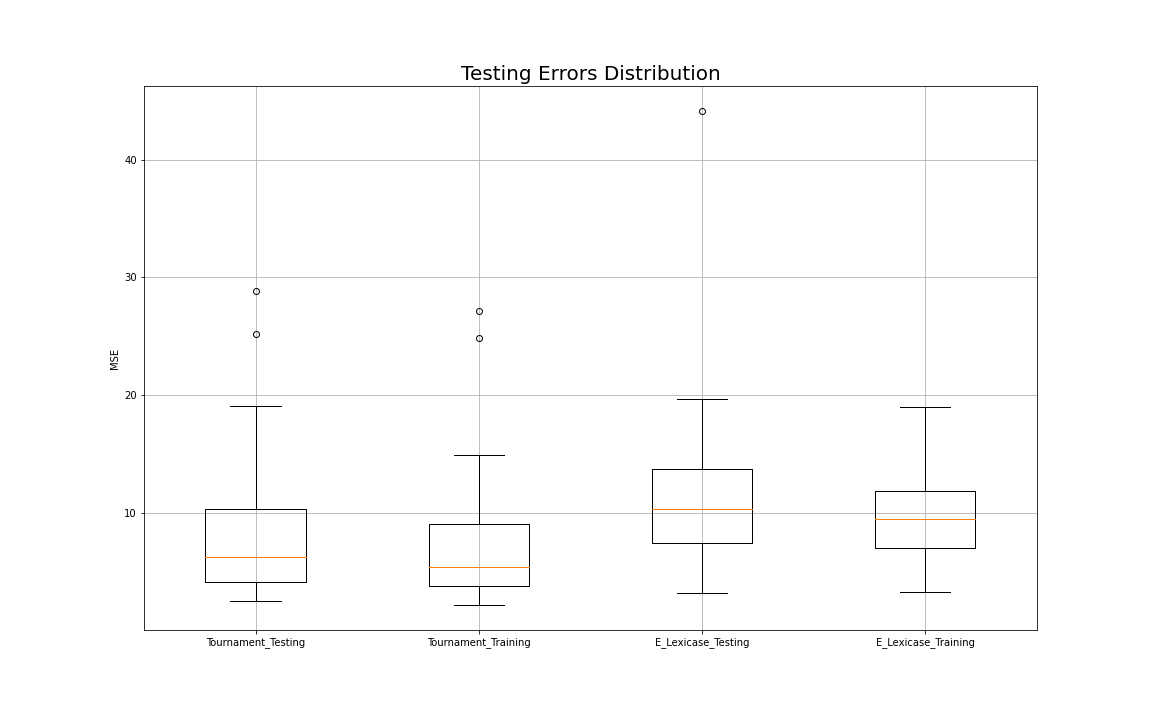
\includegraphics{./plots/mean_error_boxplot_all.png}
\caption{Distribution of Errors}
\end{figure}

The four samples from figure 1 have been tested for normal distribution
by computing the D'Agostino and Pearson test (D'Agostino, 1971)
(D'Agostino and Pearson, 1973) to determine if they satisfy the
requirements of the students t-test. The results are summarized in table
8. Since not all samples test positive for a normal distribution a
Mann-Whitney U (MWU) rank sum test will be performed to test for
statistical significance between the four variables
\(tournament\_min\_training\_error\), \(tournament\_testing\_error\),
\(e-lexicase\_min\_training\_error\) and \(e-lexicase\_testing\_error\).

\begin{table}[!h]

\caption{\label{tab:unnamed-chunk-8}Normal Distribution Tests}
\centering
\resizebox{\linewidth}{!}{
\begin{tabular}[t]{lrrrl}
\toprule
\textbf{sample} & \textbf{statistic} & \textbf{p.value} & \textbf{alpha} & \textbf{normal\_distributed}\\
\midrule
tournament\_min\_training\_error & 36.146 & 0.000 & 0.05 & False\\
e-lexicase\_min\_testing\_error & 1.575 & 0.455 & 0.05 & True\\
tournament\_testing\_error & 32.503 & 0.000 & 0.05 & False\\
e-lexicase\_testing\_error & 59.135 & 0.000 & 0.05 & False\\
\bottomrule
\end{tabular}}
\end{table}

Table 9 displays the resulting p-values from computing the MWU test in a
matrix format.

\begin{table}[!h]

\caption{\label{tab:unnamed-chunk-9}Mean Error - P-Values}
\centering
\resizebox{\linewidth}{!}{
\begin{tabular}[t]{lrrrr}
\toprule
\textbf{ } & \textbf{tournament\_training\_errors} & \textbf{tournament\_testing\_errors} & \textbf{elexicase\_training\_errors} & \textbf{elexicase\_testing\_errors}\\
\midrule
tournament\_training\_errors & 1.000 & 0.309 & 0.000 & 0.000\\
tournament\_testing\_errors & 0.309 & 1.000 & 0.002 & 0.000\\
elexicase\_training\_errors & 0.000 & 0.002 & 1.000 & 0.257\\
elexicase\_testing\_errors & 0.000 & 0.000 & 0.257 & 1.000\\
\bottomrule
\end{tabular}}
\end{table}

The results show two major findings:

\begin{enumerate}
\def\labelenumi{\arabic{enumi}.}
\item
  The differences in mean fitness between tournament selection and
  \(\epsilon\)-lexicase selection are highly statistical significant
  even if considering an \(\alpha\) of 0.01. For the given symbolic
  regression task tournament selection achieves a better mean
  performance on both the training as well as the testing data set than
  \(\epsilon\)-lexicase selection. These findings contradict the
  hypothesis \(H0_{1}\) described in subsection 3.1 and are contrary to
  some of the research that was summarized in subsections 2.1 and
  2.3.(La Cava, Spector and Danai, 2016) (La Cava \emph{et al.}, 2017).
\item
  The differences in mean fitness between \(min\_training\_error\) and
  \(testing\_error\) are not statistically significant for both
  selection algorithms. If comparing the mean training error to the mean
  testing error, the p-values only computes to 0.309 for tournament
  selection and to 0.257 for \(\epsilon\)-lexicase selection. These
  findings fail to reject \(H0_{2}\), based on the obtained results we
  can not find evidence that both algorithms demonstrate a significantly
  different performance between the training data and the previously
  unseen testing data.
\end{enumerate}

To further examine the generalization behavior of both selection
operators I plotted the mean fitness scores for both algorithms over the
total number of 100 generations in figure 2. Figure 2 shows that both
algorithms show little visual evidence of over fitting which would
result in a growing gap between between \(min\_training\_error\) and
\(testing\_error\) in the final stages of the evolutionary optimization.
For \(\epsilon\)-lexicase selection a small gap can be observed starting
at around the 90.th generation, while the minimum training error slowly
converges a small increase in the testing error can be observed. Based
on the limited amount of collected data, it is questionable if this
small sign of over fitting can be interpreted as a weak indicator for an
inferior generalization behavior of \(\epsilon\)-lexicase in comparison
to tournament selection.

Figure 2 also shows a visual representation of the described overall
performance benefit of using tournament selection instead of
\(\epsilon\)-lexicase selection for the chosen symbolic regression task.
It can be observed that at all stages of the evolution tournament
selection based GP achieves a lower mean error for both data sets.

\begin{figure}
\centering
\includegraphics{./plots/mean_error_combined.png}
\caption{Mean Errors}
\end{figure}

In a final step I analyze the growth behavior for both GP systems to
determine if differences in program size can be observed based on
selection operators. Figure 3 visualizes the average size of individuals
inside the population as well as the average size of the best performing
individual for each generation and both GP systems.

\begin{figure}
\centering
\includegraphics{./plots/size_subplotted.png}
\caption{Mean Size}
\end{figure}

Both subplots display a very similar behavior that is common for GP, we
observe a strong trend for solutions to grow in size with each
additional generation that is concluded. Another observation that can be
made is that the best solutions of each generation almost always have a
larger size than the population average. On first impression, the
differences between both selection operators appears to be
insignificant. Again, I conducted a MWU test to test for statistical
differences in the underlying distribution of sizes measured during the
experiment.

The resulting p-values of the MWU test are summarized in table 10.

\begin{table}[!h]

\caption{\label{tab:unnamed-chunk-10}Mean Size - P-Values}
\centering
\resizebox{\linewidth}{!}{
\begin{tabular}[t]{lrrrr}
\toprule
\textbf{ } & \textbf{tournament\_elite\_size} & \textbf{elexicase\_elite\_size} & \textbf{tournament\_avg\_size} & \textbf{elexicase\_avg\_size}\\
\midrule
tournament\_elite\_size & 1.000 & 0.858 & 0.533 & 0.652\\
elexicase\_elite\_size & 0.858 & 1.000 & 0.764 & 0.682\\
tournament\_avg\_size & 0.533 & 0.764 & 1.000 & 0.992\\
elexicase\_avg\_size & 0.652 & 0.682 & 0.992 & 1.000\\
\bottomrule
\end{tabular}}
\end{table}

None of the differences in mean size are statistically significant.
Again, based on the results obtained in my experiment, the evidence
produced fails to reject the null hypothesis \(H0_{3}\) that selection
has no significant effect on differences in program size. It should be
noted that the configuration of both GP algorithm did include two
mechanisms that place limitations on the growth behavior of the
individual solutions to avoid excessive bloating (see sub section
3.2.4).

\hypertarget{conclusion}{%
\section{Conclusion}\label{conclusion}}

The objective of this research project has been to answer the question
if the choice between two commonly used parent selection operators,
tournament selection and \(\epsilon\)-lexicase selection, significantly
influences the generalization behavior of GP for symbolic regression
tasks.

The results obtained from my experiment did not demonstrate any
statistically significant differences in generalization, both GP systems
achieve a slightly lower mean error if evaluated for the training data
sets than if evaluated for the unseen fitness cases of the testing data
set. The mean differences between testing and training errors did not
show statistical significance differences for both algorithms
(summarized in table 9).

To further explore differences in generalization behavior the mean for
both algorithms training and testing error over all generations for all
50 independent runs was visualized and analyzed (see figure 2). A very
small and probably insignificant gap did show for \(\epsilon\)-lexicase
selection in the final phase of the evolutionary search, in the grand
scheme of things this approach also did not yield any clear evidence of
differences in generalization.

A final attempt to explore possible differences between both GP systems
has been to explore differences in growth behavior as an indicator for
generalization. This idea was based on the wide spread hypothesis that
increases in overall program size might be an indication of over fitting
to the training data, the concept has been discussed in sub section 2.2.
Again, based on my results I could not find statistically significant
differences in the growth behavior between both selection operators.

An interesting finding of my analysis is, that the overall performance
of tournament selection has shown to be significantly better than that
of \(\epsilon\)-lexicase selection for the selected symbolic regression
problem. This finding was rather unexpected based on the research of La
Cava, Spector and Danai (2016) and La Cava \emph{et al.} (2017) that
primarily inspired this research project in the first place.

\hypertarget{limitations-and-open-questions}{%
\section{Limitations and open
questions}\label{limitations-and-open-questions}}

I faced two major difficulties in the preparation and evaluation of this
research project:

\begin{enumerate}
\def\labelenumi{\arabic{enumi}.}
\tightlist
\item
  Configuration of evolutionary parameters
\item
  Limited computational resources
\end{enumerate}

The combination of both issues might have resulted in a significant
reduction in overall robustness of the results represented in sections 5
and 6. The performance of all evolutionary algorithms, including GP, can
be highly dependent on a large number of parameters and implementation
details. Although the series of experiments conducted in this project
are comparably simple in nature, the results achieved might still be
highly influenced by the GP configuration detailed in subsection 4.2.

To gain further insight into the differences in generalization behavior
and to address the research question with a higher level of certainty,
the experiment I conducted should be repeated for different GP
configurations. Some exemplary parameters that could drastically
influence the results of this experiment include the population size,
the total number of generations, the inclusion of elitism or the
computation of \(\epsilon\) in lexicase selection. Other factors whose
influence on generalization behavior could be important include
different methods to compute an individuals fitness (e.g.~mean absolute
error or root mean squared error), testing different variations of the
genetic operators for mutation and crossover and experimenting with
different variations of the training:testing data set split size.

Another obvious weakness of this project is that the experiment is only
based on a single symbolic regression application, the prediction of the
heating load of buildings based on a relatively small data set. To gain
further trust in the obtained results, the experiment should be repeated
for other symbolic regression tasks and data sets. It remains unknown if
the generalization behavior of both selection operators might be highly
problem specific and dependent on the data set used for training and
testing.

All limitations and shortcomings described above are also connected to
the second limitation of this research project, the limited amount of
computational resources. The total computation time consumed to run the
current experiments (50 runs, 2 algorithms, 100 generations, 500
individuals) has already been close to 24 hours on a modern, arm-based
Apple-M1 system. Even though the overall computation time could probably
be reduced by further optimization of the source code, e.g.~using tools
for parallel computation, the resources necessary to repeat the whole
experiment for different parameter configurations would certainly be
beyond the scope of this research project.

\newpage

\hypertarget{I}{%
\section*{I - References}\label{I}}
\addcontentsline{toc}{section}{I - References}

\hypertarget{refs}{}
\begin{CSLReferences}{0}{0}
\leavevmode\vadjust pre{\hypertarget{ref-DAgostino1971AnOT}{}}%
D'Agostino, R.B. (1971) {``An omnibus test of normality for moderate and
large size samples,''} \emph{Biometrika}, 58, pp. 341--348.

\leavevmode\vadjust pre{\hypertarget{ref-DAgostino1973TestsFD}{}}%
D'Agostino, R.B. and Pearson, E.S. (1973) {``Tests for departure from
normality,''} in.

\leavevmode\vadjust pre{\hypertarget{ref-Dua:2019}{}}%
Dua, D. and Graff, C. (2017) {``{UCI} machine learning repository.''}
University of California, Irvine, School of Information; Computer
Sciences. Available at: \url{http://archive.ics.uci.edu/ml}.

\leavevmode\vadjust pre{\hypertarget{ref-10.1007ux2f978-3-642-16493-4_19}{}}%
Fang, Y. and Li, J. (2010) {``A review of tournament selection in
genetic programming,''} in Cai, Z. et al. (eds.) \emph{Advances in
computation and intelligence}. Berlin, Heidelberg: Springer Berlin
Heidelberg, pp. 181--192.

\leavevmode\vadjust pre{\hypertarget{ref-DEAP_JMLR2012}{}}%
Fortin, F.-A. \emph{et al.} (2012) {``{DEAP}: Evolutionary algorithms
made easy,''} \emph{Journal of Machine Learning Research}, 13, pp.
2171--2175.

\leavevmode\vadjust pre{\hypertarget{ref-Gonalves2016AnEO}{}}%
Gonçalves, I. (2016) {``An exploration of generalization and overfitting
in genetic programming: Standard and geometric semantic approaches,''}
in.

\leavevmode\vadjust pre{\hypertarget{ref-6920034}{}}%
Helmuth, T., Spector, L. and Matheson, J. (2015) {``Solving
uncompromising problems with lexicase selection,''} \emph{IEEE
Transactions on Evolutionary Computation}, 19(5), pp. 630--643.
doi:\href{https://doi.org/10.1109/TEVC.2014.2362729}{10.1109/TEVC.2014.2362729}.

\leavevmode\vadjust pre{\hypertarget{ref-soft_sensor_gp}{}}%
Jordaan, E. \emph{et al.} (2004) {``Robust inferential sensors based on
ensemble of predictors generated by genetic programming,''} in Yao, X.
et al. (eds.) \emph{Parallel problem solving from nature - PPSN VIII}.
Berlin, Heidelberg: Springer Berlin Heidelberg, pp. 522--531.

\leavevmode\vadjust pre{\hypertarget{ref-koza_main}{}}%
Koza, J.R. (1992) \emph{Genetic programming: On the programming of
computers by means of natural selection}. Cambridge, MA, USA: MIT Press.
Available at: \url{http://mitpress.mit.edu/books/genetic-programming}.

\leavevmode\vadjust pre{\hypertarget{ref-generalisation_in_gp}{}}%
Kushchu, I. (2002) {``An evaluation of EvolutionaryGeneralisation in
genetic programming,''} \emph{Artificial Intelligence Review - AIR}, 18,
pp. 3--14.
doi:\href{https://doi.org/10.1023/A:1016379201230}{10.1023/A:1016379201230}.

\leavevmode\vadjust pre{\hypertarget{ref-https:ux2fux2fdoi.orgux2f10.48550ux2farxiv.1709.05394}{}}%
La Cava, W. \emph{et al.} (2017) {``A probabilistic and multi-objective
analysis of lexicase selection and epsilon-lexicase selection.''} arXiv.
doi:\href{https://doi.org/10.48550/ARXIV.1709.05394}{10.48550/ARXIV.1709.05394}.

\leavevmode\vadjust pre{\hypertarget{ref-epsilon_lexicase_main}{}}%
La Cava, W., Spector, L. and Danai, K. (2016) {``Epsilon-lexicase
selection for regression,''} in \emph{Proceedings of the genetic and
evolutionary computation conference 2016}. New York, NY, USA:
Association for Computing Machinery (GECCO '16), pp. 741--748.
doi:\href{https://doi.org/10.1145/2908812.2908898}{10.1145/2908812.2908898}.

\leavevmode\vadjust pre{\hypertarget{ref-open_issues_gp}{}}%
O'Neill, M. \emph{et al.} (2010) {``Open issues in genetic
programming,''} \emph{Genetic Programming and Evolvable Machines}, 11,
pp. 339--363.
doi:\href{https://doi.org/10.1007/s10710-010-9113-2}{10.1007/s10710-010-9113-2}.

\leavevmode\vadjust pre{\hypertarget{ref-Orzechowski_2018}{}}%
Orzechowski, P., Cava, W.L. and Moore, J.H. (2018) {``Where are we
now?''} in \emph{Proceedings of the genetic and evolutionary computation
conference}. {ACM}.
doi:\href{https://doi.org/10.1145/3205455.3205539}{10.1145/3205455.3205539}.

\leavevmode\vadjust pre{\hypertarget{ref-10.1007ux2f978-3-540-24621-3_22}{}}%
Paris, G., Robilliard, D. and Fonlupt, C. (2004) {``Exploring
overfitting in genetic programming,''} in Liardet, P. et al. (eds.)
\emph{Artificial evolution}. Berlin, Heidelberg: Springer Berlin
Heidelberg, pp. 267--277.

\leavevmode\vadjust pre{\hypertarget{ref-poli08:fieldguide}{}}%
Poli, R., Langdon, W.B. and McPhee, N.F. (2008) \emph{A field guide to
genetic programming}. Published via \texttt{http://lulu.com}; freely
available at \texttt{http://www.gp-field-guide.org.uk}. Available at:
\url{https://digitalcommons.morris.umn.edu/cgi/viewcontent.cgi?article=1001\&context=cs_facpubs}.

\leavevmode\vadjust pre{\hypertarget{ref-bloat_overfitting_gp}{}}%
Silva, S. and Vanneschi, L. (2009) {``Operator equalisation, bloat and
overfitting: A study on human oral bioavailability prediction,''} in
\emph{Proceedings of the 11th Annual Genetic and Evolutionary
Computation Conference, GECCO-2009}, pp. 1115--1122.
doi:\href{https://doi.org/10.1145/1569901.1570051}{10.1145/1569901.1570051}.

\leavevmode\vadjust pre{\hypertarget{ref-lexicase_first_desciption}{}}%
Spector, L. (2012) {``Assessment of problem modality by differential
performance of lexicase selection in genetic programming: A preliminary
report.''}
doi:\href{https://doi.org/10.1145/2330784.2330846}{10.1145/2330784.2330846}.

\leavevmode\vadjust pre{\hypertarget{ref-fe8fa39e88a040bbacba5a465c48043f}{}}%
Tsanas, A. and Xifara, A. (2012) {``Accurate quantitative estimation of
energy performance of residential buildings using statistical machine
learning tools,''} \emph{Energy and buildings}, 49, pp. 560--567.
doi:\href{https://doi.org/10.1016/j.enbuild.2012.03.003}{10.1016/j.enbuild.2012.03.003}.

\leavevmode\vadjust pre{\hypertarget{ref-wang_wagner_rondinelli_2019}{}}%
Wang, Y., Wagner, N. and Rondinelli, J.M. (2019) {``Symbolic regression
in materials science,''} \emph{MRS Communications}, 9(3), pp. 793--805.
doi:\href{https://doi.org/10.1557/mrc.2019.85}{10.1557/mrc.2019.85}.

\end{CSLReferences}

\hypertarget{II}{%
\section*{II - Statutory Declaration}\label{II}}
\addcontentsline{toc}{section}{II - Statutory Declaration}


\includegraphics{./private/erklaerung.pdf}\\

\end{document}
